% ===========================================================================
% ANN 期末综合并行化实验报告
% ===========================================================================
\documentclass[a4paper,11pt,UTF8]{ctexart}

\usepackage[a4paper,left=2.15cm,right=2.15cm,top=2.15cm,bottom=2.15cm]{geometry}
\usepackage{amsmath}
\usepackage{amssymb}
\usepackage{booktabs}
\usepackage{caption}
\usepackage{enumitem}
\usepackage{float}
\usepackage{graphicx}
\usepackage[hidelinks]{hyperref}
\usepackage{listings}
\usepackage{xcolor}
\usepackage{array}
\usepackage{tabularx}
\usepackage{fancyhdr}
\usepackage{tikz}
\usetikzlibrary{arrows.meta,calc,positioning,shapes.geometric}

\graphicspath{{./}{fig/}}
\setlength{\parindent}{2em}
\setlength{\parskip}{2pt}
\setlength{\textfloatsep}{8pt plus 2pt minus 2pt}
\setlength{\intextsep}{6pt plus 2pt minus 2pt}
\setlength{\abovecaptionskip}{4pt}
\setlength{\belowcaptionskip}{2pt}
\setlist{leftmargin=1.8em,itemsep=1.5pt,topsep=2pt}
\captionsetup{font=small,labelsep=quad}
\renewcommand{\arraystretch}{1.16}
\newcommand{\code}[1]{\texttt{\detokenize{#1}}}
\newcolumntype{Y}{>{\raggedright\arraybackslash}X}
\newcolumntype{C}[1]{>{\centering\arraybackslash}p{#1}}

\lstset{
  basicstyle=\ttfamily\footnotesize,
  keywordstyle=\color{blue!65!black},
  commentstyle=\color{green!40!black},
  numbers=left,
  numberstyle=\tiny,
  frame=single,
  breaklines=true,
  showstringspaces=false,
  columns=fullflexible,
  aboveskip=4pt,
  belowskip=4pt
}

\pagestyle{fancy}
\fancyhf{}
\lhead{\kaishu ANN 综合并行化实验}
\rhead{\kaishu SIMD / 多核 / MPI / GPU}
\cfoot{\thepage}
\setlength{\headheight}{14pt}
\renewcommand{\headrulewidth}{0.1pt}

\begin{document}

\begin{titlepage}
  \begin{center}
    
\includegraphics[width=0.72\textwidth]{NKU.png}\\[1.0cm]
    {\huge\kaishu 计算机学院\par}
    \vspace{0.45cm}
    {\huge\kaishu 并行程序设计期末综合实验报告\par}
    \vspace{1.45cm}
    {\Huge\kaishu ANN 近似最近邻搜索\par}
    \vspace{0.45cm}
    {\LARGE\kaishu SIMD、多核、MPI 与 GPU 架构上的综合并行化实验\par}
    \vspace{1.0cm}
    {\Large\kaishu 进阶选题：Approximate Nearest Neighbor Search\par}
    \vspace{0.18cm}
    {\Large\kaishu 新增内容：自适应 IVF-PQ 查询预算、难度分层、grouped-order 迁移验证与跨架构瓶颈归因\par}
    \vfill
    {\LARGE\kaishu 姓名：柯云超\par}
    \vspace{0.35cm}
    {\LARGE\kaishu 学号：2413575\par}
    \vspace{0.35cm}
    {\LARGE\kaishu 专业：计算机科学与技术\par}
    \vspace{0.35cm}
    {\Large\kaishu GitHub 仓库：\href{https://github.com/kyc001/parallel}{\texttt{https://github.com/kyc001/parallel}}\par}
    \vfill
    {\Large 2026 年 6 月 30 日\par}
  \end{center}
\end{titlepage}

\tableofcontents
\clearpage

% ===========================================================================
\section*{摘要}
\addcontentsline{toc}{section}{摘要}
% ===========================================================================

选这个进阶选题是因为 ANN 问题的结构特别适合把这学期学到的东西串起来——不只是"各种架构都能加速"，而是每种架构解决的是同一个搜索问题里不同位置的瓶颈。做完所有实验之后，让我印象最深的一条结论是：\textbf{ANN 优化的本质是一条瓶颈迁移链}。当你用 SIMD 把距离计算压下去，带宽墙就显现；当你加了量化减少访存，查表和候选维护就变得可见；当你上了多核并行，图搜索里的锁和尾部任务就开始拖后腿；当你上了 GPU，Top-$k$ 合并突然就变成了和矩阵乘同量级的瓶颈。这条迁移链贯穿本文的全部分析。

具体实验覆盖了 SIMD 侧的 Flat/SQ/PQ/FastScan（分别在 i9-13900H AVX2 和鲲鹏 AArch64 NEON 上），多核侧的 Pthread/OpenMP、inter/intra 粒度、IVF/IVF-PQ/HNSW、调度和虚假共享，MPI 侧的 IVF-PQ、block-HNSW、IVF+HNSW、HNSW-on-HNSW 以及阻塞/非阻塞通信，GPU 侧的 batch GEMM、cuBLAS、设备端树形 Top-$k$ 和 grouped-IVF。期末新增实验实现了一个查询难度感知的自适应 IVF-PQ 驱动（\code{adaptive_ivfpq.cc}），验证了固定参数之间存在可利用的 query 难度差异，同时把 GPU grouped-IVF 的分组思想迁移回 CPU，发现单独分组反而变慢，只有与自适应预算结合才能降低延迟——这个"不能直接照搬"的结论本身就是一个跨架构融合实验应当有的认知。

代表性数字：SQ-AVX2（$p=100$）在 Recall@10 = 0.99995 时达到 427.01 us/query，相对串行 Flat 加速 10.71 倍；IVF-PQ Pthread 线程池 16 线程达到 57.61 us/query，Recall@10 = 0.95945；MPI block-HNSW 8 ranks 在 Windows 上达到 188.03 us/query 且 Recall@10 = 1.00000；GPU cublas\_tree 全量批量扫描达到 83.24 us/query，Recall@10 = 0.99995；期末新增 conservative+grouped 配置在 8 线程下达到 186.54 us/query，Recall@10 = 0.96520。

% ===========================================================================
\section{选题动机与工作边界}
% ===========================================================================

\subsection{为什么选 ANN 进阶选题}

做前四次实验的时候，SIMD、多核、MPI 和 GPU 各自有一套评价框架，看起来是独立的问题。选 ANN 进阶选题的原因，就是想逼自己把这些架构放在同一个问题里看——到底是哪个环节决定了端到端性能，换一种并行方式能解决前一种方式遗留的瓶颈，还是会引入新的问题？

当然，进阶选题要求也明确说了"不是做的内容越多越好，每个内容浅尝辄止不会得到高分"。我理解这个意思是：应该对同一个问题有足够深度的探索，而不是把四次作业的结论剪贴到一起。因此本文的组织原则是：以 ANN 系统的在线查询流水线为主线，把不同架构的优化映射到同一组代价项上，分析它们分别在压低哪一项、引入了哪些新问题，再把期末新增实验放在"前序工作自然延伸"的位置，而不是单独一章硬凑"新内容"。

\subsection{平时作业与新增内容声明}

按作业要求，新增内容需要超过 20\% 并明确标注。表 \ref{tab:old_new_work} 列出了工作来源。

\begin{table}[H]
  \centering\footnotesize
  \begin{tabularx}{\textwidth}{p{2.6cm}Y Y}
    \toprule
    模块 & 平时作业工作 & 期末新增内容 \\
    \midrule
    问题建模 & 各次实验分别使用 DEEP100K、Recall@10、平均延迟，但没有把四类架构放到统一代价模型下比较。 & 统一在线查询代价分解 $T=T_{\mathrm{score}}+T_{\mathrm{candidate}}+T_{\mathrm{topk}}+T_{\mathrm{sync}}+T_{\mathrm{transfer}}$，图 \ref{fig:ann_pipeline} 的系统流水线，以及各架构分别"主要压哪一项"的系统性分析。 \\
    SIMD & Flat/SQ/PQ/FastScan 实现与对比，AVX2 与 NEON 两平台 VTune 证据，汇编分析。 & 将 SIMD 重新定位到"距离计算与量化压缩"环节，解释从 DRAM-bound 到 compute/LUT-bound 的瓶颈迁移，与后续架构的候选规模和调度策略打通。 \\
    Pthread/OpenMP & inter/intra 粒度、多种调度策略、IVF/IVF-PQ/HNSW、虚假共享和 P/E-core 亲和性实验。 & 抽象出"查询级并行优先"的多核设计原则，并与期末自适应预算的 8 线程驱动实验衔接。 \\
    MPI & IVF-PQ、block-HNSW 等多算法分布式搜索，参数扫描，阻塞/非阻塞通信，跨平台结果。 & 系统解释固定长度候选协议的正确性证明，通信占比归因，以及"当前主瓶颈是 rank-local 搜索而非通信"的量化说明。 \\
    GPU & batch GEMM、cuBLAS、树形 Top-$k$、grouped-IVF、CUDA event 分段、cuobjdump/PTX/SASS 静态分析。 & 将 GPU 结果放回"batch + 规则矩阵 + 设备端合并"的统一模型，并以 grouped-IVF 思想迁移 CPU 实验作为期末新增研究的动机。 \\
    期末新增 & 无前序对应。 & \code{adaptive_ivfpq.cc}：固定/自适应预算$\times$分组/原始顺序$\times$动态/静态调度的 12 配置完整对照；hard/medium/easy 难度分层统计；跨架构迁移结论。 \\
    综合分析 & 各次作业单独给结论。 & 跨架构代表性结果表，profiling 证据到优化决策的映射，以及"瓶颈迁移链"的统一解释。 \\
    \bottomrule
  \end{tabularx}
  \caption{平时作业工作与期末新增内容划分}
  \label{tab:old_new_work}
\end{table}

新增内容不只是字数意义上的"20\%"。从研究贡献角度看，期末新增实验补充了一类前序作业没有回答的问题：\textit{在固定架构（Pthread IVF-PQ）之内，用 query 难度感知的方式重新分配搜索预算，是否能同时改善 recall 和延迟？当 GPU 的分组组织思想被搬回 CPU 时，哪些条件让它有效、哪些条件让它失效？} 这两个问题的答案不能从前序实验直接推导，需要新的 benchmark。

% ===========================================================================
\section{ANN 问题：高维搜索的核心困难}
% ===========================================================================

\subsection{问题定义与评价指标}

给定 $N$ 个 $d$ 维 base 向量
\[
X=\{x_1,x_2,\ldots,x_N\}\subset \mathbb{R}^{d},
\]
以及查询向量 $q\in\mathbb{R}^{d}$，精确 $k$NN 的目标是找出 $X$ 中距离 $q$ 最近的 $k$ 个向量。实验使用 DEEP100K 数据集：$N=100000$，$d=96$，查询数 $Q=2000$，$k=10$。评价指标统一为
\[
\mathrm{Recall@10}=\frac{|KNN(q)\cap KANN(q)|}{10}
\]
和每查询平均延迟（us/query）。GPU 实验额外区分 online 延迟和 wall 延迟（含显存拷贝和索引构建）。

这里有一个值得先讲清楚的事：Recall@10 和延迟之间永远存在折中，但它的\textbf{形状}取决于你用的是哪类算法。Flat 精确扫描在 Recall@10 = 1.0 的同时代价最高；IVF 类算法通过控制 $nprobe$ 可以在低召回和高召回之间移动，代价曲线更陡；HNSW 的曲线形状不同，在中等 \code{efSearch} 下很容易达到高 recall，再往上提升则代价急剧攀升。整个学期的实验都在探索这条 recall-latency 曲线：能不能在同样的 recall 下用更快的实现，或者在同样的延迟下获得更高的 recall。

\subsection{一次查询的代价分解}

为了能把四类架构放在同一个框架里讨论，我把一次在线查询的耗时分解成：
\[
T(q)=T_{\mathrm{score}}(q)+T_{\mathrm{candidate}}(q)+T_{\mathrm{topk}}(q)+T_{\mathrm{sync}}(q)+T_{\mathrm{transfer}}(q).
\]
$T_{\mathrm{score}}$ 是计算向量距离或得分的成本；$T_{\mathrm{candidate}}$ 是通过索引（IVF probe、PQ ADC、HNSW 图扩展）生成候选集的成本；$T_{\mathrm{topk}}$ 是从候选集中维护和提取最终 Top-$k$ 的成本；$T_{\mathrm{sync}}$ 是线程同步、MPI gather/merge 和负载尾部等同步代价；$T_{\mathrm{transfer}}$ 仅在 GPU 或 MPI 路径存在显式数据移动时计入。

这个分解的价值不在于公式本身，而在于用它问具体问题：SIMD 向量化主要压低了哪一项？多核 inter-query 并行摊薄的是哪一项的固定成本？MPI 通信到底占 $T(q)$ 的多少比例？GPU Top-$k$ 没有优化时，压低 $T_{\mathrm{score}}$ 会怎样？后文的每一组分析都会回到这个分解。

\subsection{四类加速杠杆与系统流水线}

整学期实验可以归纳出四类加速杠杆：
\begin{enumerate}
  \item \textbf{更快的距离计算}：压低 $T_{\mathrm{score}}$ 的常数，包括 Flat-SIMD、SQ/PQ/FastScan 以及 CUDA GEMM。
  \item \textbf{更少的候选访问}：通过 IVF、HNSW 等索引改变 $T_{\mathrm{candidate}}$ 的规模，从 $O(N)$ 降到更小的 $O(nprobe \cdot N/nlist)$ 或图扩展量。
  \item \textbf{更多查询同时处理}：摊薄 $T_{\mathrm{sync}}$ 和调度固定成本，包括 inter-query 多核、GPU batch 和 MPI rank-local 并行。
  \item \textbf{更高效的合并调度}：降低 $T_{\mathrm{topk}}+T_{\mathrm{sync}}$，包括线程私有堆、MPI 固定长度候选协议和 GPU 设备端树形 Top-$k$。
\end{enumerate}

图 \ref{fig:ann_pipeline} 展示了这些杠杆在 ANN 系统流水线中的位置。不同架构在同一条流水线上的切入点不同——这也是为什么它们能互相补充而不是互相替代。

\begin{figure}[H]
  \centering
\resizebox{\textwidth}{!}{%
  \begin{tikzpicture}[
    node distance=0.75cm,
    box/.style={draw=black!55, rounded corners=2pt, align=center, minimum height=0.82cm, font=\small, fill=blue!5},
    opt/.style={draw=black!45, rounded corners=2pt, align=center, font=\scriptsize, fill=orange!10},
    arr/.style={-{Latex[length=2.2mm]}, thick, draw=black!65}
  ]
    \node[box, minimum width=2.3cm] (data) {Base 向量\\DEEP100K};
    \node[box, right=of data, minimum width=2.45cm] (offline) {离线索引\\SQ/PQ/IVF/HNSW};
    \node[box, right=of offline, minimum width=2.35cm] (query) {在线查询\\batch / stream};
    \node[box, right=of query, minimum width=2.65cm] (score) {距离或得分\\SIMD / GEMM};
    \node[box, right=of score, minimum width=2.5cm] (cand) {候选集\\probe / graph};
    \node[box, right=of cand, minimum width=2.2cm] (topk) {Top-$k$\\merge};
    \node[box, right=of topk, minimum width=2.2cm] (eval) {Recall@10\\latency};
    \draw[arr] (data) -- (offline);
    \draw[arr] (offline) -- (query);
    \draw[arr] (query) -- (score);
    \draw[arr] (score) -- (cand);
    \draw[arr] (cand) -- (topk);
    \draw[arr] (topk) -- (eval);
    \node[opt, below=0.6cm of score, xshift=-1.0cm] (simd) {SIMD\\向量化距离};
    \node[opt, below=0.6cm of cand] (mc) {Pthread/OpenMP\\query 或候选并行};
    \node[opt, below=0.6cm of topk] (mpi) {MPI\\局部分区 + 全局合并};
    \node[opt, below=0.6cm of query, xshift=1.0cm] (gpu) {GPU\\batch GEMM + device Top-$k$};
    \draw[arr, dashed] (simd) -- (score);
    \draw[arr, dashed] (mc) -- (cand);
    \draw[arr, dashed] (mpi) -- (topk);
    \draw[arr, dashed] (gpu) -- (score);
  \end{tikzpicture}
}
  \caption{ANN 综合并行化流水线与不同架构的主要切入点}
  \label{fig:ann_pipeline}
\end{figure}

有一个容易犯的错误需要在这里提前说明：不同架构的优化并不都是独立叠加的。如果 $T_{\mathrm{score}}$ 已经被 SIMD 压到很低，继续加 SIMD 指令的回报递减；如果 $T_{\mathrm{topk}}$ 成为主瓶颈，优化 $T_{\mathrm{score}}$ 几乎没有帮助。所以判断"下一步该优化哪里"必须靠实际 profiling，而不是凭直觉。这也是本文把 profiling 结果单独作为一个分析层次的原因。

% ===========================================================================
\section{SIMD 实验：第一次碰到内存墙}
% ===========================================================================

\subsection{从 Flat-AVX2 开始：向量化加速了什么}

做 SIMD 实验之前，我以为把 Flat 的内积循环从标量改成 AVX2 就能得到接近理论峰值的加速——毕竟一条 \code{_mm256_dp_ps} 一次能处理 8 个 float，理论上应该有 8 倍提速。实际结果是 Flat-AVX2 在 i9-13900H 上相对串行 Flat 只有 2.60x 加速（4571.62 → 1756.11 us/query）。

用 VTune Top-Down 分析 Flat-AVX2 的 P-core 热循环，Back-End Bound 达到 71.4\%，其中 Memory Bound 占 47.7\%。这说明循环里的向量化乘加指令并不慢，真正的瓶颈是把 $N=100000$ 个 96 维 float32 向量从内存读进来——无论 AVX2 多快，数据总线的吞吐上限决定了最终速度。Flat 精确扫描在计算上是"容易的"，在访存上却是固定代价的，这个认知贯穿了后续所有量化实验。

\subsection{量化的意义：换数据表示，不只是换指令}

为了真正压下延迟，我实现了标量量化（SQ）和乘积量化（PQ）两类两阶段方案：

\textbf{SQ 两阶段}：把每维 float32 量化为 uint8，粗排阶段在压缩表示上算近似距离，筛出 top-$p$ 后回到原始 float32 精排。粗排数据体积降至 1/4，但关键是访问的字节数也降至 1/4，这才是带宽压力下降的原因。VTune 显示 SQ 的 Memory Bound 从 47.7\% 降到了约 8.7\%，同时 Retiring 占比上升——说明计算通路开始变成主限制。

\textbf{PQ 两阶段}：把 96 维向量分成 $M$ 个子空间，每个子空间在线为当前 query 构建 LUT，通过 ADC（Asymmetric Distance Computation）累加近似距离。PQ 进一步压缩了粗排的数据体积，但引入了查表开销。

核心参数是精排预算 $p$：$p$ 越小，延迟越低但可能漏掉真实近邻；$p$ 越大，召回率趋近于 Flat，但精排代价回升。从表 \ref{tab:simd_results} 可以看出，SQ-AVX2 在 $p=100$ 时以 Recall@10 = 0.99995 达到 427.01 us/query，加速比从纯向量化的 2.60x 一跃到 10.71x。这 10x+ 的提升中，"用 AVX2 算得更快"只贡献了其中一部分，更大的贡献来自"用压缩表示读的字节数更少"。

\begin{table}[H]
  \centering\footnotesize
  \begin{tabular}{llrrr}
    \toprule
    平台 & 方法 & Recall@10 & Latency (us) & 相对 baseline \\
    \midrule
    i9 AVX2 & 串行 Flat & 0.99995 & 4571.62 & 1.00x \\
    i9 AVX2 & Flat-AVX2 & 0.99995 & 1756.11 & 2.60x \\
    i9 AVX2 & SQ-AVX2, $p=100$ & 0.99995 & 427.01 & 10.71x \\
    i9 AVX2 & PQ-AVX2, $p=1000$ & 0.98330 & 761.99 & 6.00x \\
    Kunpeng NEON & 串行 Flat & 0.99995 & 16120.74 & 1.00x \\
    Kunpeng NEON & Flat-SIMD & 0.99995 & 5821.16 & 2.77x \\
    Kunpeng NEON & SQ-SIMD, $p=100$ & 0.99995 & 2422.68 & 6.65x \\
    Kunpeng NEON & PQ-SIMD, $p=1000$ & 0.98355 & 1984.35 & 8.12x \\
    \bottomrule
  \end{tabular}
  \caption{SIMD 核心结果（i9-13900H AVX2 与鲲鹏 NEON）}
  \label{tab:simd_results}
\end{table}

鲲鹏 NEON 的趋势与 i9 AVX2 高度一致：Flat-SIMD 只有 2.77x，SQ/PQ 后提升到 6--8x。鲲鹏的绝对延迟更高，部分原因是 NEON 宽度为 128-bit 而 AVX2 为 256-bit，另一部分原因是内存总线吞吐不同。但两平台都能说明同一个事实：SIMD 向量化的作用不能脱离"被处理数据的表示"单独评估。

\subsection{FastScan：把查表搬进寄存器}

FastScan 是 PQ 路线的进一步优化。标准 PQ ADC 的内层循环对每个子空间做 LUT 查表，查表结果写到内存再累加；FastScan 使用 4-bit code（$K_s=16$），把 16 个距离值压进一个小整数 LUT，利用 AVX2 的 \code{_mm256_shuffle_epi8} 在寄存器内完成查表，同时批量处理 32 个候选向量。核心思想是：把从 L1/L2 cache 读 LUT 的操作变成"LUT 住在 256-bit 寄存器里"。

图 \ref{fig:simd_fastscan_tradeoff} 展示了 FastScan 相对标准 PQ 在不同精排预算下的 recall-latency 折中。可以看到当 $p$ 较小（粗排主导时），FastScan 的优势更明显；随着 $p$ 增大，精排的 float32 计算开始主导，FastScan 在 ADC 阶段的节省比例就相对变小了。这说明 FastScan 的价值不只是"换更快的指令"，而是"在候选规模较小、粗排占比较大时，把查表代价真正压到底"。

\begin{figure}[H]
  \centering
  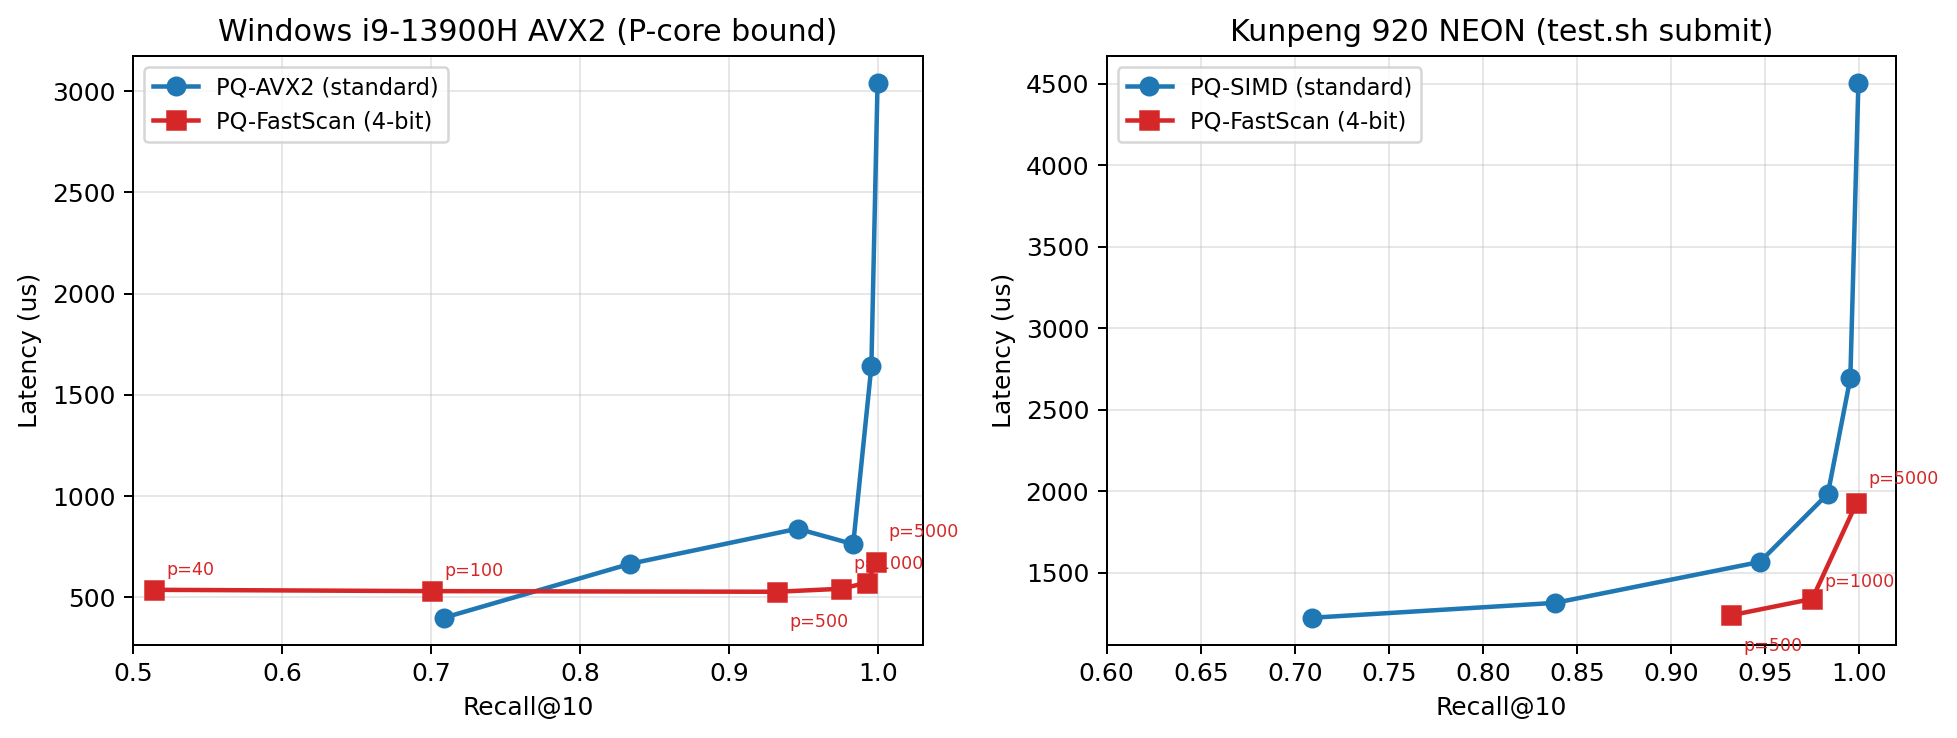
\includegraphics[width=0.74\textwidth]{simd_fastscan_tradeoff.png}
  \caption{FastScan 与标准 PQ 在不同精排预算下的 recall-latency 折中（i9-13900H AVX2 平台）}
  \label{fig:simd_fastscan_tradeoff}
\end{figure}

\subsection{SIMD 实验对期末报告的意义}

做完 SIMD 实验，我理解了一件后来在多核、MPI 和 GPU 实验中反复验证的事：\textbf{$p$（精排预算）是 ANN 召回-延迟折中里最通用的旋钮}。无论之后用哪种并行架构，只要基于两阶段检索，都绕不开"粗排筛多少、精排算多少"这个决策。期末新增实验的"自适应预算"正是把这个旋钮从全局固定值变成了 per-query 的动态分配——后文会展开这部分。

SIMD 实验对架构融合的另一个贡献是：理清了"底层计算核"的角色。无论上层是 Pthread/OpenMP、MPI 还是 GPU，真正执行距离计算的仍然是这些 SIMD 内核。多核实验的 inter-query 路径每个线程都在调用同一套 SIMD 计算函数；MPI 每个 rank 内的 local search 也继承了 SIMD 数据布局；GPU 则把这个层换成了 cuBLAS/CUDA kernel。因此本节不是与后文并列的"第几章"，而是整个 ANN 计算栈的基础层。

% ===========================================================================
\section{多核实验：inter-query 为什么比 intra-query 更稳}
% ===========================================================================

\subsection{两种并行粒度的设计选择}

进入多核实验时，我面对的第一个设计问题是：任务应该在哪个层次上划分？两种选择都有直觉上的道理：

\textbf{intra-query 并行}：把一条 query 的搜索工作拆给多线程。每个线程处理 base 向量的一段、或若干 IVF list、或 HNSW 的若干入口点，最后合并局部 Top-$k$。优点是单条 query 延迟更低，适合低延迟服务场景；缺点是候选集要合并，需要线程间同步，且 query 内部的候选数量（如 IVF 的 $nprobe$ 个 list）不一定能均匀填满所有线程。

\textbf{inter-query 并行}：不同线程各处理不同 query，每条 query 的内部流程完全独立。批量 $Q$ 个 query 均匀分给 $T$ 个线程，每线程完成 $Q/T$ 条 query 后写到结果数组中预先分配好的槽位。优点是线程间完全无锁（结果槽按 query 预分配）、任务粒度均匀；缺点是对单条 query 的延迟没有帮助，只提高了吞吐。

本次实验以批量 $Q=2000$ 评测，吞吐比单条 query 延迟更重要。事实证明 inter-query 是正确选择，但我在做实验之前并不确定，于是系统地测了 intra-query。

\subsection{intra-query 的实际问题}

以 IVF-PQ（$nlist=16$，$nprobe=4$）为例，整个搜索过程分为"选 $nprobe$ 个最近 centroid、扫描这些 list、对候选精排、维护 Top-$k$"四步。如果用 intra-query 并行，可以把 4 个 list 分给最多 4 个线程；但如果线程数是 16，其中 12 个线程会直接空转。即使 $nprobe$ 增大，候选列表的不均匀性（不同 list 里的向量数可能差很大）也会产生负载尾部，让某个线程严重拖延整体。

从代价模型看，intra-query 的总时间近似为：
\[
T_{\mathrm{intra}} \approx \frac{C_{\mathrm{scan}}}{T} + C_{\mathrm{local\ heap}} + C_{\mathrm{merge}} + C_{\mathrm{sync}}.
\]
当 $T > nprobe$ 时，$C_{\mathrm{scan}}/T$ 没有继续降低，而 $C_{\mathrm{merge}}$ 和 $C_{\mathrm{sync}}$ 仍然存在，实际延迟反而可能上升。

HNSW 的 intra-query 更加棘手。图搜索有路径依赖——下一步要访问哪个节点，取决于当前最佳候选——这是天然的串行结构。多入口点并行（不同线程从不同入口出发）确实能改善召回率，但它更接近"用更多计算换更高 recall"，而不是"用更多线程提速"。VTune hotspot 也显示 \code{searchBaseLayer} 和 \code{pthread_mutex_lock} 同时出现在热路径上，说明优先队列的锁争用在 intra-query HNSW 场景中不可忽略。

\subsection{inter-query 的稳定性}

相比之下，inter-query 的代价模型要干净得多：
\[
T_{\mathrm{inter}} \approx \frac{Q}{T} \cdot C_{\mathrm{search}} + C_{\mathrm{schedule}},
\]
其中 $C_{\mathrm{schedule}}$ 是任务调度的额外开销（Pthread dynamic 是原子 \code{fetch\_add}，线程池是条件变量唤醒，OpenMP 是 schedule chunk 管理）。当 $Q=2000$ 时，$Q/T$ 对于 $T=16$ 来说是 125，任务粒度足够大，调度开销完全可以摊薄。

表 \ref{tab:multicore_best} 列出了各算法在本地 i9 平台上的 Pthread/OpenMP 最优结果。所有高召回最优点均来自 inter-query 路径。

\begin{table}[H]
  \centering\footnotesize
  \begin{tabular}{llrrr}
    \toprule
    算法 & 最优变体 & 线程数 & Recall@10 & Latency (us) \\
    \midrule
    Flat & Pthread dynamic inter & 16 & 0.99995 & 298.95 \\
    SQ & Pthread dynamic inter & 16 & 0.99995 & 86.53 \\
    PQ & OpenMP inter & 16 & 0.98335 & 131.97 \\
    FastScan & Pthread dynamic inter & 16 & 0.97525 & 125.81 \\
    IVF & Pthread pool inter & 16 & 0.96225 & 104.67 \\
    IVF-PQ & Pthread pool inter & 16 & 0.95945 & 57.61 \\
    HNSW & baseline 单线程 & 1 & 0.96865 & 65.48 \\
    \bottomrule
  \end{tabular}
  \caption{Windows i9 平台 Pthread/OpenMP 最优结果（inter-query 路径）}
  \label{tab:multicore_best}
\end{table}

IVF-PQ Pthread pool inter 在 16 线程时达到 57.61 us/query，是所有多核配置中最快的。HNSW 单线程 65.48 us/query 已经很快，但它的并行化空间有限：增大 \code{efSearch} 可以提升 recall，但代价会线性增长；多入口点并行是 recall-latency 折中，不是加速路径。

\subsection{调度细节：schedule 不是小事}

我做了一组 OpenMP schedule 参数扫描，结果出乎我预料。在 16 线程 Flat 搜索中，\code{guided,8} 达到 287.87 us/query，而 \code{static,256} 是 428.74 us/query，差距约 1.5x。这个差距的来源是：每条 query 在不同算法下的计算时间并不完全均匀（特别是 HNSW 和 IVF，候选数量随 query 而变），\code{static} 切块太大时某些线程会先完成然后空等，\code{guided} 和 \code{dynamic} 能把小块任务及时分给空闲线程。反过来，块太小时调度开销本身会上升，所以最优 chunk size 需要实测而不能硬猜。

虚假共享（false sharing）实验则说明了另一个容易被忽略的问题：多个线程在写结果时，如果结果槽紧邻且跨越同一 cache line，即使逻辑上没有争用，CPU 也会因 cache coherence protocol 引发不必要的写冲突。按 query 预分配结果数组并对齐到 cache line，是 inter-query 路径能稳定扩展到 16 线程的前提之一。

图 \ref{fig:multicore_tradeoff_curves} 汇总了多核实验中主要算法的 recall-latency 曲线，直观地展示了 HNSW、IVF-PQ、SQ 等各自覆盖的质量区间。

\begin{figure}[H]
  \centering
  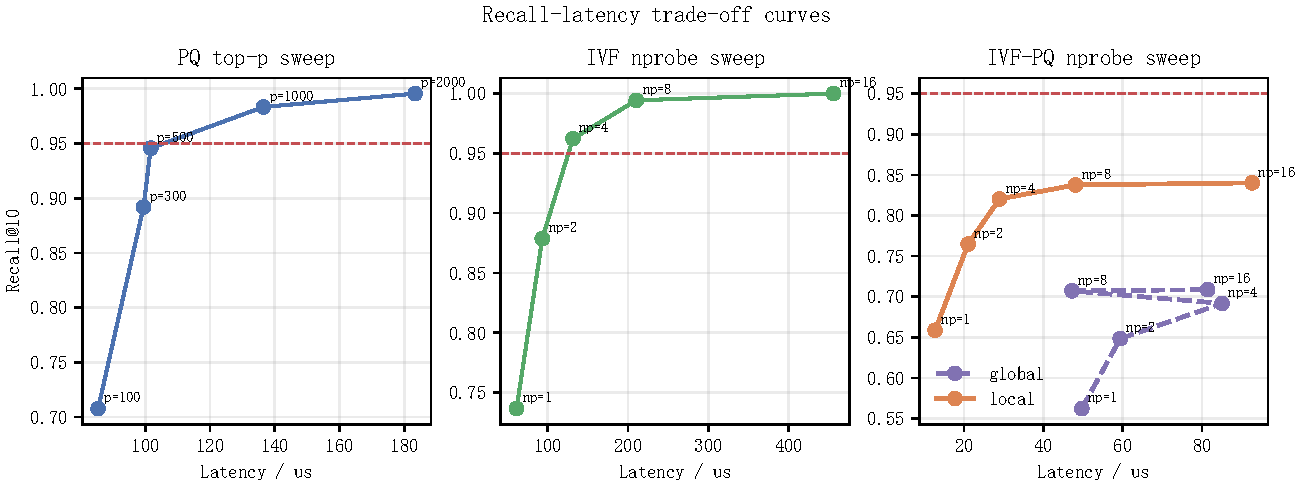
\includegraphics[width=0.76\textwidth]{multicore_tradeoff_curves.pdf}
  \caption{Pthread/OpenMP 实验中代表性算法的 recall-latency 曲线（Windows i9-13900H，16 线程）}
  \label{fig:multicore_tradeoff_curves}
\end{figure}

\subsection{多核实验对期末报告的意义}

多核实验最终让我理解了"并行粒度必须匹配任务结构"。批量 $Q=2000$ 的查询是天然可并行的，每条 query 独立，没有数据依赖——inter-query 完美利用了这个结构。而 intra-query 试图在单条 query 内部并行，反而打破了 IVF 和 HNSW 各自的局部局部性。

这个教训在期末新增实验中有直接体现：自适应预算驱动仍然用 8 线程 inter-query 作为基础并行架构，新增的是 per-query 的预算分配逻辑。跨架构迁移的 grouped-order 实验也以 inter-query 为前提，只是在调度上让相同 centroid 分组的 query 连续处理，以改善 cache 局部性。

% ===========================================================================
\section{MPI 实验：通信根本不是瓶颈}
% ===========================================================================

\subsection{分布式 ANN 的设计直觉}

做 MPI 实验之前，我以为分布式 ANN 的主要挑战是通信：$Q=2000$ 条 query 每条都要广播给所有 rank，每个 rank 完成本地搜索后再把结果汇总到 root，中间的数据传输应该是性能瓶颈。

实验做完之后，这个预判几乎完全错了。

\subsection{固定长度候选协议：通信为什么可以很小}

MPI 路径的设计遵循"owner computes"原则：base shard 分给哪个 rank，就由该 rank 构建局部索引，完成局部搜索，并返回本地的固定长度候选。整个 MPI 层只处理四件事：\code{Scatterv} 分发 base 分片、\code{Bcast} 广播所有 query、每个 rank 回传本地 top-$k$ 候选、root 合并全局 Top-$k$。

候选协议的正确性有一个简单的证明：若某向量 $v$ 属于全局 top-$k$，则它必然属于其所在 rank 的局部 top-$k$。原因是：如果它不是本 rank 的局部 top-$k$，则同一 rank 内至少已有 $k$ 个向量比它更近，这些向量同样进入了全局候选空间，矛盾。因此每个 rank 只需回传每条 query 的 $k=10$ 个 \code{(distance, global\_id)} 对，总通信量为：
\begin{itemize}
  \item query 广播：$Q \cdot d \cdot 4 = 2000 \times 96 \times 4 \approx 750$ KiB
  \item 每 rank 结果回传：$Q \cdot k \cdot (4+8) = 2000 \times 10 \times 12 \approx 234$ KiB
\end{itemize}

与 rank 内部的 IVF-PQ 扫描或 HNSW 图遍历相比，这个量级几乎可以忽略不计。

\subsection{实验结果与归因}

表 \ref{tab:mpi_cross} 列出了主要 MPI 实验的结果。可以看到，在 8 ranks $\times$ 2 OpenMP threads 的配置下，通信与合并延迟（Comm 列）多数在 2--4 us/query，而本地搜索延迟（Max local 列）在百 us 量级。通信占总延迟的比例不超过 2\%。

\begin{table}[H]
  \centering\scriptsize
  \begin{tabularx}{\textwidth}{p{2.9cm}p{2.4cm}C{1.35cm}C{1.45cm}C{1.45cm}C{1.15cm}Y}
    \toprule
    平台路径 & 算法 & Recall@10 & Latency & Max local & Comm & 解释 \\
    \midrule
    Windows MS-MPI & IVF-PQ & 0.96515 & 297.56 & 295.04 & 2.52 & 倒排量化适合中等召回。 \\
    Windows MS-MPI & block-HNSW & 1.00000 & 188.03 & 185.86 & 2.17 & 本地图质量高，合并代价小。 \\
    Windows MS-MPI & IVF+HNSW & 0.96450 & 245.05 & 241.75 & 3.29 & 两级索引有额外筛选开销。 \\
    Windows MS-MPI & HNSW-on-HNSW & 0.99995 & 764.21 & 761.49 & 2.71 & 高覆盖但全 block 探测代价大。 \\
    Kunpeng PBS & IVF-PQ & 0.96515 & 498.41 & 494.64 & 3.77 & ARM 环境下 recall 一致，时间受平台影响。 \\
    Kunpeng PBS & block-HNSW & 1.00000 & 803.68 & 800.99 & 2.69 & 图遍历在 ARM 更慢，通信仍不是主因。 \\
    \bottomrule
  \end{tabularx}
  \caption{MPI 跨平台代表结果，8 ranks $\times$ 2 OpenMP threads，延迟单位 us/query}
  \label{tab:mpi_cross}
\end{table}

图 \ref{fig:mpi_comm_balance} 展示了 MPI 实验中通信与 rank 本地搜索的负载分布，直观体现了本地搜索时间几乎完全主导端到端延迟的事实。

\begin{figure}[H]
  \centering
  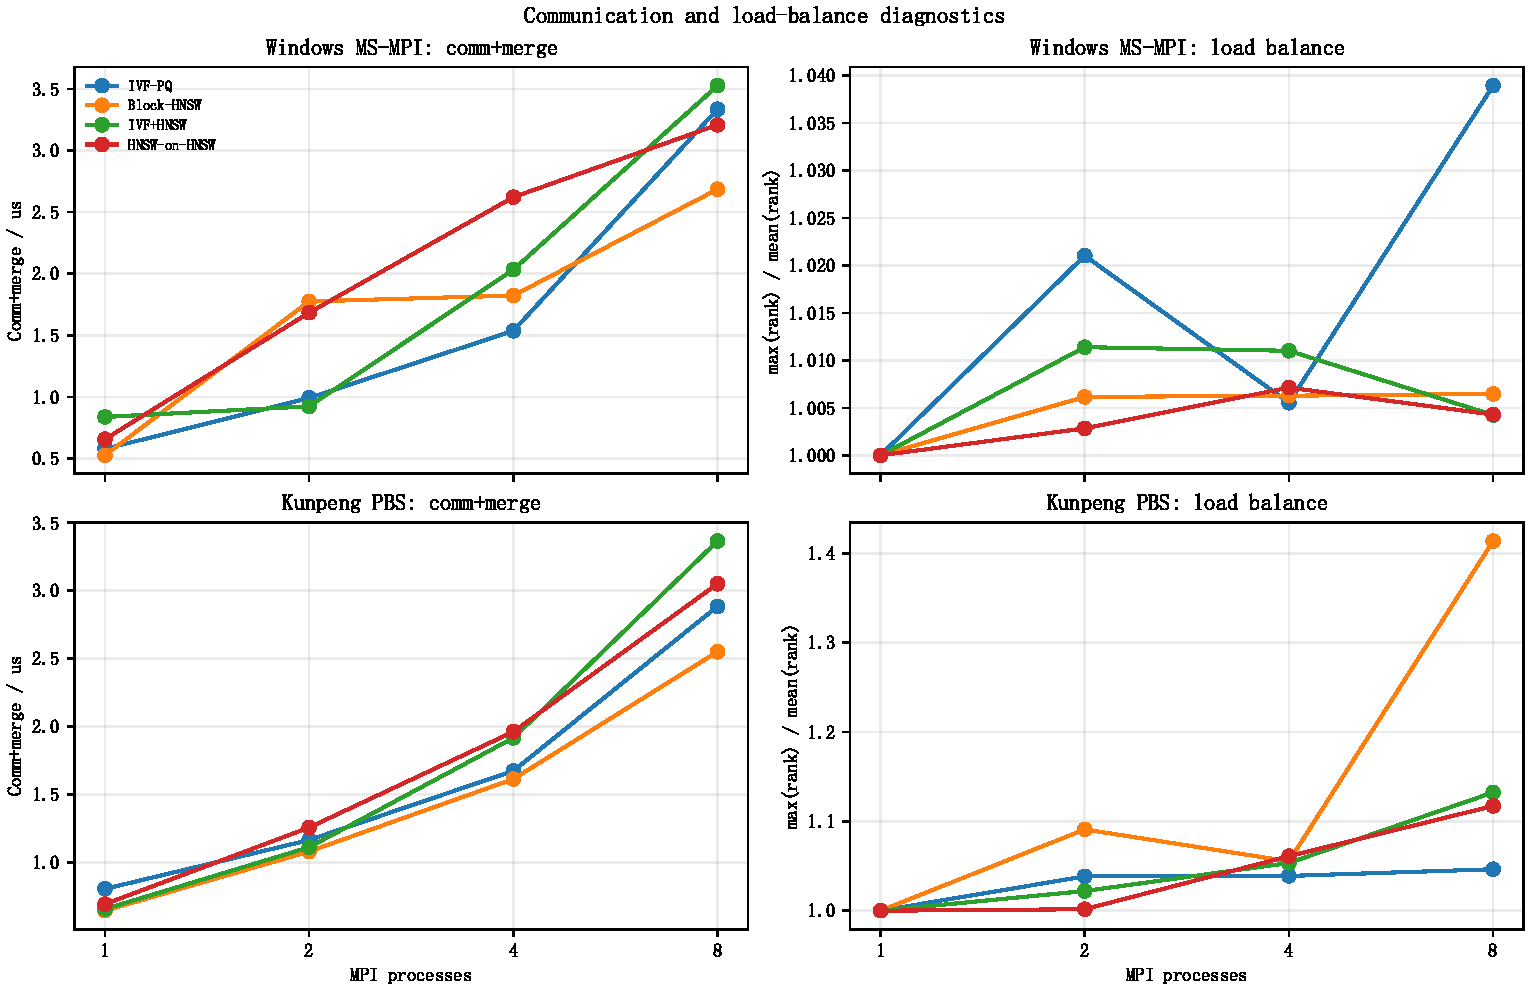
\includegraphics[width=0.76\textwidth]{mpi_comm_balance.pdf}
  \caption{MPI 通信与 rank-local 搜索延迟对比（8 ranks，各算法配置）}
  \label{fig:mpi_comm_balance}
\end{figure}

从跨平台结果还可以检验正确性：相同算法参数在 Windows MS-MPI 与鲲鹏 PBS 上 Recall@10 完全一致（IVF-PQ 均为 0.96515，block-HNSW 均为 1.00000），说明 global id 映射和 root merge 没有破坏 Top-$k$ 语义。两平台的延迟差异来自硬件、编译器和队列负载，不能被解读为"MPI 算法在某平台更好"。

\subsection{$nprobe$ 参数扫描：更说明 local search 是主角}

表 \ref{tab:nprobe_sweep} 展示了随着 $nprobe$ 增大，主要增加的是本地搜索时间，通信时间几乎保持不变。

\begin{table}[H]
  \centering\footnotesize
  \begin{tabular}{rrrrr}
    \toprule
    $nprobe$ & Recall@10 & Latency (us) & Max local (us) & Comm+merge (us) \\
    \midrule
    1 & 0.74535 & 190.79 & 187.30 & 3.49 \\
    2 & 0.89125 & 280.69 & 277.33 & 3.36 \\
    4 & 0.96515 & 334.60 & 331.11 & 3.49 \\
    8 & 0.99330 & 428.70 & 424.33 & 4.37 \\
    16 & 0.99995 & 561.90 & 558.31 & 3.59 \\
    \bottomrule
  \end{tabular}
  \caption{MPI IVF-PQ $nprobe$ 参数扫描（Windows MS-MPI，8 ranks $\times$ 2 threads）}
  \label{tab:nprobe_sweep}
\end{table}

这组数据有一个直接的设计含义：如果在当前 MPI 路径上想继续优化，应该先优化 rank 内的局部搜索（例如改进 IVF-PQ 数据布局、引入更高效的 SIMD 量化内核），而不是继续调优通信 API 或改非阻塞模式。阻塞/非阻塞对比实验也验证了这一点：当前单 batch 设计下，\code{MPI\_Ibcast}/$\code{MPI\_Waitall}$ 相比 \code{MPI\_Bcast} 的收益极为有限，只有引入多 batch pipeline（让下一批 broadcast 与当前批搜索重叠）才能让非阻塞通信真正发挥价值。

\subsection{MPI 实验对期末报告的意义}

MPI 实验最清晰地证明了一件事：\textbf{通信量受候选协议设计控制，而不是问题规模本身决定的}。同样是 $Q=2000$ 条 query、8 个 rank，如果把每个 rank 的完整候选池（可能几千个向量）回传 root，通信量会急剧增大；固定长度候选协议把回传量固定为 $Q \cdot P \cdot k$，与 $nprobe$、候选池大小无关。这个设计和期末新增的自适应预算有一个共通之处：都是在"全局合并"和"局部搜索"之间找接口协议，让两侧可以独立优化。

% ===========================================================================
\section{GPU 实验：Top-k 才是真正的意外瓶颈}
% ===========================================================================

\subsection{用矩阵乘法重新理解 Flat 扫描}

做 GPU 实验之前，我对 GPU 的预期是：矩阵乘法是 GPU 的强项，用 cuBLAS 把所有 query 与所有 base 向量的内积写成一次 SGEMM，应该能取得很大加速。这个预期在 score 阶段是正确的，但实验很快说明了：score 只是第一步，Top-$k$ 同样重要，而且更容易被低估。

GPU Flat 的计算形式为：
\[
S = B Q^\top, \quad B \in \mathbb{R}^{N \times D}, \quad Q^\top \in \mathbb{R}^{D \times M},
\]
其中 $M$ 是 batch 大小，$S_{ij}$ 是第 $i$ 个 base 向量与第 $j$ 个 query 的内积。这个形式同时利用了 base 维度和 query 维度上的并行，适合 tiled GEMM。但如果把完整 $N \times M$ 的 score 矩阵传回 CPU 排序，$N=100000$，$M=2000$ 时矩阵大小约 762 MiB，PCIe 传输加上主机侧排序会成为新的主瓶颈。因此实验采用的策略是：按 query chunk 计算 score tile，然后立即在设备端完成 Top-$k$，只回传每条 query 的 10 个 id 和距离。

\subsection{score 与 Top-k 的双瓶颈}

表 \ref{tab:gpu_results} 列出了各种 GPU 配置的分段计时结果，这是本节最核心的证据。

\begin{table}[H]
  \centering\scriptsize
  \begin{tabular}{lrrrrrr}
    \toprule
    模式 & Recall@10 & Online us & Wall us & Score ms & Topk ms & Result ms \\
    \midrule
    gemm 2000 & 0.99990 & 237.63 & 331.43 & 240.08 & 226.56 & 6.68 \\
    gemm\_tree 2000 & 0.99995 & 165.05 & 256.43 & 229.94 & 91.92 & 6.75 \\
    cublas 2000 & 0.99990 & 145.27 & 233.59 & 69.47 & 214.49 & 5.02 \\
    cublas\_tree 2000 & 0.99995 & 83.24 & 162.95 & 70.71 & 89.44 & 5.18 \\
    ivf 16/4 & 0.96275 & 468.19 & 688.25 & 3.34 & 922.68 & 8.22 \\
    ivf\_grouped 16/4 & 0.96280 & 145.32 & 375.75 & 87.72 & 64.04 & 84.73 \\
    ivf\_grouped 16/8 & 0.99345 & 189.90 & 419.52 & 143.18 & 89.95 & 89.16 \\
    \bottomrule
  \end{tabular}
  \caption{GPU batch ANN 实验分段计时均值（RTX 4060 Laptop，CUDA，batch=2000）}
  \label{tab:gpu_results}
\end{table}

从这张表可以看出几条关键链条：

\textbf{链条 1：手写 GEMM → cuBLAS 只优化了 score}。\code{gemm} 到 \code{cublas} 的在线延迟从 237.63 降到 145.27 us，主要原因是 score 从 240.08 ms 降到 69.47 ms（约 3.5x）。但 Top-$k$ 仍为 214.49 ms，几乎和 score 等量。两项加在一起，cuBLAS 只带来了有限的端到端收益。

\textbf{链条 2：优化 Top-k 才解锁了 cuBLAS 的真正收益}。\code{cublas\_tree} 同时用 cuBLAS 做 score 和设备端树形归并做 Top-$k$，score 70.71 ms、Top-$k$ 89.44 ms，端到端 83.24 us/query，相比 \code{cublas} 提升接近 1.75x。如果只优化 GEMM 而不管 Top-$k$，整体只能达到 145.27 us；只有两者同步优化，才真正释放了 batch GEMM 的价值。

这个双瓶颈现象事先并不显而易见，但事后解释并不难：GPU 上的 Top-$k$ 合并需要排序或堆操作，这是不规则的内存访问和分支密集型计算，远不如 GEMM 适合 GPU 的流式处理架构。基础版的 Top-$k$ 每个 block 处理一条 query，最后由线程 0 顺序合并各线程的局部候选，这个顺序合并步骤是严重的串行尾部。改成树形归并后，每轮减半参与线程数，共享内存利用率提高，才真正把合并代价压了下来。

\subsection{grouped-IVF：组织候选，不只是选择候选}

GPU IVF 实验揭示了另一个有趣的现象。表 \ref{tab:gpu_ivf_compare} 对比了 per-query IVF 和 grouped-IVF 在相同 $nprobe$ 下的结果：

\begin{table}[H]
  \centering\footnotesize
  \begin{tabular}{lrrr}
    \toprule
    模式 & $nprobe$ & Recall@10 & Online latency (us) \\
    \midrule
    grouped-IVF & 2 & 0.87340 & 94.01 \\
    grouped-IVF & 4 & 0.96280 & 145.32 \\
    grouped-IVF & 8 & 0.99345 & 189.90 \\
    per-query IVF & 4 & 0.96275 & 468.19 \\
    per-query IVF & 8 & 0.99345 & 789.29 \\
    \bottomrule
  \end{tabular}
  \caption{GPU IVF 组织方式对比（$nprobe=4$ 时 recall 几乎相同，延迟相差 3.2x）}
  \label{tab:gpu_ivf_compare}
\end{table}

$nprobe=4$ 时，两者 Recall@10 几乎相同（0.96280 vs 0.96275），但延迟差距达到 3.2x（145.32 vs 468.19 us）。这个差距来自哪里？

per-query IVF 让每个 query 按自己的 $nprobe$ 个 list 顺序扫描，不同 query 访问不同 list，GPU warp 内的线程执行不同的内存访问路径，出现严重的 warp divergence 和不规则的全局内存访问。grouped-IVF 先把 batch 内 query 按它们的最近 centroid 分桶，把访问同一 list 的 query 聚到一起，再对每个 list 内的 query 和候选向量做小批矩阵运算。这样，原本不规则的逐 query list 扫描，变成了更接近矩阵计算的规则内存访问。代价是多了分桶、重排和结果重组的额外开销（Result ms 从 5 ms 上升到 84 ms），但候选扫描阶段的效率大幅提升。

这个"组织候选比选择候选更重要"的思想，成为期末新增实验的核心动机之一。

\subsection{PTX/SASS 静态分析}

除运行时分段计时外，实验还通过 \code{cuobjdump} 导出了 PTX 和 SASS，查看寄存器使用量和 shared memory 分配情况。结果显示 tree Top-$k$ kernel 的寄存器压力较大（每线程约 40+ 寄存器），这会在 occupancy 和 ILP 之间产生折中——寄存器用得多，每个 SM 能同时驻留的 warp 数变少，但每个 warp 内的 ILP 更高。当前 batch 尺寸下这个折中是有利的，但如果 batch 减小或 query 数减少，occupancy 不足可能会变成新的限制。

\subsection{GPU 实验对期末报告的意义}

GPU 实验最重要的教训是：\textbf{GPU 加速不是把 CPU 循环直接搬到 device 上}，而是需要同时考虑 batching（有足够的并行度）、数据组织（让候选扫描尽量规则）和设备端合并（Top-$k$ 不能让主机做）。grouped-IVF 的思想——"把访问同一 list 的 query 聚到一起"——能不能也用在 CPU 侧的 Pthread 调度中？这个问题推动了期末新增实验的设计。

% ===========================================================================
\section{期末新增实验：查询难度感知与跨架构迁移验证}
% ===========================================================================

\subsection{出发点：固定预算是否浪费了资源}

做完前四次实验后，我注意到一个一直被忽略的问题：无论是 SIMD 实验还是多核实验，IVF-PQ 的 $nprobe$ 和精排预算 $p$ 始终是对所有 query 固定的。但直觉上，不同 query 的"搜索难度"差异很大——有些 query 距离最近的 centroid 非常近，落在某个簇内部，较小的 $nprobe$ 就能找到真实近邻；有些 query 处在多个簇的边界附近，可能需要探测更多 list 才能不漏掉近邻。

用固定预算对待所有 query，很可能是在"简单 query"上浪费资源，在"困难 query"上又分配不足。这个想法催生了期末新增实验的核心问题：\textbf{能否用一个无监督的、可解释的难度指标来重新分配搜索预算，在不改变总体计算量的前提下提升整体召回率？}

\subsection{centroid margin 作为难度指标}

我用最近和次近 centroid 的距离差来衡量 query 难度：
\[
m(q) = d(q, c_2) - d(q, c_1),
\]
其中 $c_1, c_2$ 分别是最近和次近 centroid。$m(q)$ 大意味着 $q$ 明确落在某个簇内，它对 $c_1$ 的 list 的依赖很强，搜索一两个 list 基本足够；$m(q)$ 小意味着 $q$ 处于两个簇的交界处，漏掉 $c_2$ 的 list 很可能漏召回真实近邻。

这个指标不需要 ground truth 标签，也不需要任何机器学习训练——只需要查询向量与 centroid 的距离，这在 IVF 搜索的第一步就已经算好了，几乎没有额外开销。

实验用前 256 个 query 的 margin 估计 $1/3$ 和 $2/3$ 分位阈值，得到 $\tau_1 = 0.03368$，$\tau_2 = 0.08289$。全体 2000 个 query 按阈值分为 hard/medium/easy 三类，数量分别为 623/569/808。三种自适应策略如表 \ref{tab:adaptive_policy} 所示。

\begin{table}[H]
  \centering\scriptsize
  \begin{tabularx}{\textwidth}{p{2.6cm}C{2.2cm}C{2.2cm}C{2.2cm}Y}
    \toprule
    策略 & hard ($nprobe, p$) & medium ($nprobe, p$) & easy ($nprobe, p$) & 设计意图 \\
    \midrule
    conservative & $(5,1000)$ & $(4,1000)$ & $(3,800)$ & 固定中档附近微调，降低 easy 成本，给 hard 适度加预算。 \\
    aggressive & $(8,1500)$ & $(4,1000)$ & $(2,500)$ & 把预算更激进地从 easy 转移到 hard。 \\
    recall-oriented & $(8,1500)$ & $(5,1000)$ & $(4,1000)$ & 追求更高召回，保留较高 easy/medium 预算。 \\
    \bottomrule
  \end{tabularx}
  \caption{期末新增自适应策略定义，单元格为 $(nprobe, p)$}
  \label{tab:adaptive_policy}
\end{table}

核心控制流如清单 \ref{lst:adaptive_ivfpq} 所示，代码位于 \code{ann-final/experiments/adaptive_ivfpq.cc}，复用前序 IVF-PQ 的索引、PQ 扫描和精排函数。

\begin{lstlisting}[language=C++,caption=自适应 IVF-PQ 预算控制流程（简化）,label={lst:adaptive_ivfpq}]
for each query q:
    centroid_dists = distance(q, all_centroids)
    c1, c2 = two_nearest_centroids(centroid_dists)
    margin = dist(q, c2) - dist(q, c1)
    if margin <= tau_low:
        budget = high_budget      // hard query：边界附近
    else if margin <= tau_high:
        budget = mid_budget
    else:
        budget = low_budget       // easy query：落在簇内部
    probes = nearest_centroids(q, budget.nprobe)
    coarse = scan_ivfpq_lists(probes, budget.rerank_p)
    result = exact_rerank(coarse, k=10)
\end{lstlisting}

\subsection{实验结果：预算感知确实有效}

表 \ref{tab:adaptive_ivfpq} 列出了本地 Windows i9、8 个 Pthread、$nlist=16$、DEEP100K 前 2000 个 query 的完整对照矩阵（来自 \code{adaptive\_ivfpq\_20260630.csv}）。

\begin{table}[H]
  \centering\scriptsize
  \begin{tabularx}{\textwidth}{p{3.05cm}C{1.05cm}C{1.28cm}C{1.05cm}C{1.15cm}C{1.35cm}Y}
    \toprule
    策略 & Rec. & Latency & 平均 $nprobe$ & 平均 $p$ & 平均扫描 & 说明 \\
    \midrule
    固定低档 $2/500$ & 0.86940 & 148.43 & 2.00 & 500.00 & 15984 & easy 尚可，hard 召回明显不足。 \\
    固定中档 $4/1000$ & 0.95945 & 229.06 & 4.00 & 1000.00 & 28710 & 同驱动固定参数基线。 \\
    固定近邻档 $5/1000$ & 0.97300 & 324.82 & 5.00 & 1000.00 & 34697 & 增加 probe 后召回提升，延迟显著上升。 \\
    固定高档 $8/1500$ & 0.99265 & 340.32 & 8.00 & 1500.00 & 52971 & 高召回上限，扫描量最大。 \\
    adaptive conservative & 0.96520 & 217.38 & 3.91 & 919.20 & 28107 & 比固定中档召回提升 0.00575，延迟降约 5.1\%。 \\
    adaptive aggressive & 0.97115 & 216.00 & 4.44 & 953.75 & 31102 & hard 获得高预算，整体召回继续提升。 \\
    adaptive recall-oriented & 0.98420 & 301.43 & 5.53 & 1155.75 & 37910 & 介于固定近邻档和固定高档之间。 \\
    conservative + grouped & 0.96520 & 186.54 & 3.91 & 919.20 & 28107 & 自适应预算叠加 grouped-order 后延迟最低。 \\
    \bottomrule
  \end{tabularx}
  \caption{期末新增 IVF-PQ 预算实验（Windows i9，8 Pthread，$nlist=16$，延迟单位 us/query）}
  \label{tab:adaptive_ivfpq}
\end{table}

conservative 策略相对固定中档，Recall@10 从 0.95945 提升到 0.96520，同时延迟从 229.06 us 降到 217.38 us——两项指标都改善了。这个结果说明固定中档在 easy query 上存在"过度投资"，把节省下来的预算转移给 hard query 后，整体 recall 提升而总计算量几乎持平。aggressive 策略在相近延迟下进一步把 recall 推到 0.97115。

图 \ref{fig:adaptive_recall_latency} 直观地展示了这些配置在 recall-latency 平面上的分布。

\begin{figure}[H]
  \centering
  \resizebox{0.92\textwidth}{!}{% Generated by gen_adaptive_fig.py from adaptive_ivfpq_20260630.csv
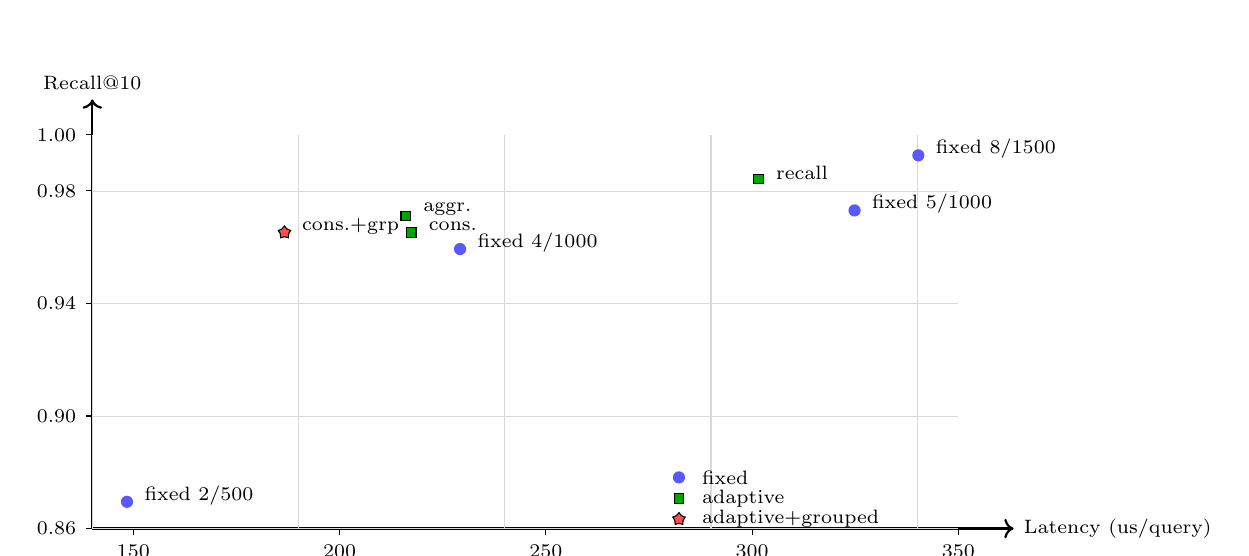
\begin{tikzpicture}[font=\scriptsize]
  \draw[->,thick] (0,0) -- (11.7,0) node[right] {Latency (us/query)};
  \draw[->,thick] (0,0) -- (0,5.45) node[above] {Recall@10};
  \draw (0.52,0) -- (0.52,-0.08) node[below] {150};
  \draw (3.14,0) -- (3.14,-0.08) node[below] {200};
  \draw (5.76,0) -- (5.76,-0.08) node[below] {250};
  \draw (8.38,0) -- (8.38,-0.08) node[below] {300};
  \draw (11.00,0) -- (11.00,-0.08) node[below] {350};
  \draw (0,0.00) -- (-0.08,0.00) node[left] {0.86};
  \draw (0,1.43) -- (-0.08,1.43) node[left] {0.90};
  \draw (0,2.86) -- (-0.08,2.86) node[left] {0.94};
  \draw (0,4.29) -- (-0.08,4.29) node[left] {0.98};
  \draw (0,5.00) -- (-0.08,5.00) node[left] {1.00};
  \draw[black!15] (0,0) grid[xstep=2.619,ystep=1.428] (11,5);
  \fill[blue!65] (0.44,0.34) circle (2.2pt);
  \node[anchor=west] at (0.54,0.42) {fixed 2/500};
  \node[star,star points=5,fill=red!70,draw=black,inner sep=1.1pt] at (2.44,3.76) {};
  \node[anchor=west] at (2.54,3.84) {cons.+grp};
  \draw[fill=green!65!black,draw=black] (3.92,3.91) rectangle (4.04,4.03);
  \node[anchor=west] at (4.08,4.05) {aggr.};
  \draw[fill=green!65!black,draw=black] (3.99,3.70) rectangle (4.11,3.82);
  \node[anchor=west] at (4.15,3.84) {cons.};
  \fill[blue!65] (4.67,3.55) circle (2.2pt);
  \node[anchor=west] at (4.77,3.63) {fixed 4/1000};
  \draw[fill=green!65!black,draw=black] (8.40,4.38) rectangle (8.52,4.50);
  \node[anchor=west] at (8.56,4.52) {recall};
  \fill[blue!65] (9.68,4.04) circle (2.2pt);
  \node[anchor=west] at (9.78,4.12) {fixed 5/1000};
  \fill[blue!65] (10.49,4.74) circle (2.2pt);
  \node[anchor=west] at (10.59,4.82) {fixed 8/1500};
  \fill[blue!65] (7.45,0.65) circle (2.2pt); \node[anchor=west] at (7.62,0.65) {fixed};
  \draw[fill=green!65!black,draw=black] (7.39,0.32) rectangle (7.51,0.44); \node[anchor=west] at (7.62,0.38) {adaptive};
  \node[star,star points=5,fill=red!70,draw=black,inner sep=1.1pt] at (7.45,0.12) {}; \node[anchor=west] at (7.62,0.12) {adaptive+grouped};
\end{tikzpicture}
}
  \caption{期末新增 IVF-PQ 实验的 recall-latency 分布（各配置来自同一驱动的 CSV 输出）}
  \label{fig:adaptive_recall_latency}
\end{figure}

\subsection{难度分层统计：margin 的解释力}

表 \ref{tab:difficulty_bins} 列出了各策略在 hard/medium/easy 三类 query 上的分层统计。

\begin{table}[H]
  \centering\scriptsize
  \begin{tabularx}{\textwidth}{p{3.1cm}C{1.1cm}C{1.1cm}C{1.1cm}C{1.45cm}C{1.45cm}Y}
    \toprule
    策略 & hard Rec. & mid Rec. & easy Rec. & hard 扫描 & easy 扫描 & 解释 \\
    \midrule
    固定中档 & 0.91830 & 0.96116 & 0.98998 & 27360 & 30225 & 同一预算对 hard 不够，对 easy 偏多。 \\
    固定高档 & 0.98427 & 0.99490 & 0.99752 & 51436 & 54411 & 召回最高，但所有 query 承担高扫描量。 \\
    adaptive conservative & 0.94398 & 0.96116 & 0.98441 & 33333 & 24129 & 少量预算从 easy 转移给 hard。 \\
    adaptive aggressive & 0.98427 & 0.96116 & 0.96807 & 51436 & 17583 & hard 提升最大，但 easy 损失更明显。 \\
    adaptive recall-oriented & 0.98427 & 0.97592 & 0.98998 & 51436 & 30225 & 保留 easy 质量，成本介于中高档之间。 \\
    \bottomrule
  \end{tabularx}
  \caption{查询难度分层统计（hard/medium/easy 数量分别为 623/569/808）}
  \label{tab:difficulty_bins}
\end{table}

最值得关注的是：固定中档在 easy query 上已达到 Recall@10 = 0.98998，在 hard query 上只有 0.91830，两者差距超过 0.07。aggressive 策略把 hard recall 推到了 0.98427，但 easy recall 降到了 0.96807。这说明 centroid margin 不是一个随机指标，它确实在区分"需要更多预算"和"可以节省预算"的 query 上有实质性的解释力。

\subsection{CPU 侧 grouped-order 实验：直接照搬为什么不行}

把 GPU grouped-IVF 的思想迁移到 CPU，最直接的做法是：把 2000 个 query 按最近 centroid 排序，让访问同一 list 的 query 连续处理，以期改善 Pthread 调度中的 cache 局部性（相邻 query 访问相同 list，list 数据在 cache 中更可能驻留）。

但实验结果给了我一个意外：表 \ref{tab:group_schedule} 显示，单独把固定中档 query 按 centroid 分组，延迟反而从 229.06 us 上升到 250.72 us（动态调度）或 305.99 us（静态调度）。原因是固定中档下所有 query 的预算相同，分组后 hard query 和 easy query 的工作量完全一样，分组只带来了额外的 query 重排开销，却没有改善负载均衡。静态调度下更差的原因是，按 centroid 分组后查询的执行时间分布变得更不均匀（相邻 query 都访问同一批 list，竞争同一批 cache），静态切块放大了这种不均衡。

\begin{table}[H]
  \centering\footnotesize
  \begin{tabularx}{\textwidth}{p{3.4cm}C{1.4cm}C{1.4cm}C{1.2cm}C{1.45cm}Y}
    \toprule
    配置 & 调度 & query 顺序 & Rec. & Latency & 观察 \\
    \midrule
    固定中档 & dynamic & original & 0.95945 & 229.06 & 同驱动基线。 \\
    固定中档 & dynamic & grouped & 0.95945 & 250.72 & 只做分组反而变慢。 \\
    固定中档 & static & original & 0.95945 & 268.16 & 静态调度放大尾部不均衡。 \\
    固定中档 & static & grouped & 0.95945 & 305.99 & 分组+静态调度最差。 \\
    conservative & dynamic & original & 0.96520 & 217.38 & 自适应预算优于固定中档。 \\
    conservative & dynamic & grouped & 0.96520 & 186.54 & 分组+自适应预算，延迟最低。 \\
    conservative & static & original & 0.96520 & 220.64 & 静态接近但略慢于动态调度。 \\
    \bottomrule
  \end{tabularx}
  \caption{CPU 侧 grouped-order 与调度策略对照实验}
  \label{tab:group_schedule}
\end{table}

然而当 grouped-order 与 conservative 自适应预算结合时，延迟从 217.38 us 降到了 186.54 us。原因是：conservative 策略让 easy query 的预算更小、hard query 的预算更大，而分组后相邻 query 恰好也有相似的 centroid，局部性改善使 hard query 在访问多个 list 时能从 cache 复用更多数据。两种优化的叠加效果超过了各自的单独效果。

这组实验让我相信：\textbf{跨架构迁移不是复制设计的表面形式，而是要理解背后的驱动机制}。GPU grouped-IVF 的目标是减少 warp divergence 和不规则内存访问；CPU grouped-order 的目标则是改善 Pthread 调度的 cache 局部性和负载均衡。两者的驱动机制不同，因此单独使用分组在 CPU 上失效，但与预算感知结合后才产生协同效果。

% ===========================================================================
\section{跨架构融合分析}
% ===========================================================================

\subsection{从分散实验到统一框架：同一个环节的四种实现}

做完所有实验之后，最让我有收获感的一步是把各次作业的优化"对齐"到 ANN 系统的同一个环节上。表 \ref{tab:same_stage_compare} 把四类架构放回 ANN 流水线的五个环节中对比，揭示了各架构在同一问题上选择不同切入点的原因。

\begin{table}[H]
  \centering\scriptsize
  \begin{tabularx}{\textwidth}{p{2.3cm}p{2.7cm}p{2.7cm}p{2.7cm}Y}
    \toprule
    ANN 环节 & SIMD/单核 & Pthread/OpenMP & MPI & GPU \\
    \midrule
    距离/得分计算 & AVX2/NEON FMA、整数 SQ、PQ ADC LUT。 & 每线程独立调用相同 SIMD kernel；向量化在线程层之下。 & 每 rank 本地调用相同 SIMD/OpenMP kernel；跨 rank 无共享。 & batch GEMM/cuBLAS，把 query 和 base 组成矩阵乘法，充分利用 tensor core。 \\
    候选集缩减 & SQ/PQ/FastScan 通过压缩表示减少精排候选数量。 & IVF/IVF-PQ/HNSW 在单机多线程内控制候选规模；inter-query 不改变每条 query 的候选数。 & 每 rank 只搜索自己的 shard，总候选数按 rank 数减少；局部 Top-$k$ 通过协议恢复全局正确性。 & IVF grouped 按 probe list 组织 batch，使候选扫描更规则，核心是组织方式而非候选数量。 \\
    Top-$k$ 合并 & 单线程堆或按插入维护，结果直接写回。 & 每 query 私有结果槽；intra-query 需合并线程局部堆。 & rank 0 合并 $P \times k$ 固定长度候选；$O(QPk)$ 排序。 & 设备端树形归并，只回传 $k$ 个结果；主机侧合并几乎可忽略。 \\
    调度/负载均衡 & cache blocking 和精排预算 $p$。 & static/dynamic/pool、schedule、cache line 隔离。 & rank 负载尾部决定关键路径；固定长度协议保证 root 合并均匀。 & query chunk、probe 分桶、kernel launch 粒度和 shared memory 复用。 \\
    期末新增关联 & centroid margin 最终调用 SIMD/IVF-PQ 距离核。 & 自适应预算在 8 线程 Pthread 驱动中验证；grouped-order 需与动态调度配合。 & 可把 margin 作为每 rank 的预算控制策略继续扩展。 & grouped-IVF 思想迁移到 CPU 需要重新匹配调度与预算分配。 \\
    \bottomrule
  \end{tabularx}
  \caption{同一 ANN 流水线环节在四类架构上的实现对照}
  \label{tab:same_stage_compare}
\end{table}

这张表的价值不在于"把四列填满"，而在于它揭示了一个核心规律：\textbf{不同架构在同一环节选择的优化维度不同，因此它们是互补的，而不是替代关系}。SIMD 改变了数据表示（量化）；多核改变了调度粒度（inter-query）；MPI 改变了数据分区（rank shard）；GPU 改变了 batch 组织方式（tiled GEMM + 设备端 Top-$k$）。在理想情况下，这四类优化可以叠加——例如 MPI 的每个 rank 内部使用 SIMD 量化 kernel，再在 rank 内用 OpenMP inter-query 并行，最后汇总到 root。

\subsection{跨架构代表性结果对照}

表 \ref{tab:representative_results} 把各架构的代表性结果放在一起，不作跨平台硬件排名，而是展示每条技术路线在 recall-latency 平面上的位置。

\begin{table}[H]
  \centering\scriptsize
  \begin{tabularx}{\textwidth}{p{1.35cm}p{2.55cm}p{2.75cm}C{1.15cm}C{1.35cm}Y}
    \toprule
    架构 & 平台 & 代表方法 & Rec. & Latency & 主要说明 \\
    \midrule
    SIMD & i9-13900H AVX2 & SQ-AVX2, $p=100$ & 0.99995 & 427.01 & 相对串行 Flat 10.71x，高召回低延迟最优点。 \\
    SIMD & Kunpeng NEON & PQ-SIMD, $p=1000$ & 0.98355 & 1984.35 & 趋势与 AVX2 一致，绝对延迟更高。 \\
    多核 & Windows i9 & IVF-PQ Pthread pool inter, 16T & 0.95945 & 57.61 & inter-query 最稳定，线程池减少调度开销。 \\
    多核 & Windows i9 & HNSW baseline, 1T & 0.96865 & 65.48 & 图索引单线程已快，并行空间有限。 \\
    期末新增 & Windows i9 & adaptive conservative + grouped, 8T & 0.96520 & 186.54 & 预算感知与分组协同，同驱动最优点。 \\
    MPI & Windows MS-MPI & block-HNSW, 8 ranks $\times$ 2T & 1.00000 & 188.03 & 局部图后全局合并，通信约 2.17 us。 \\
    MPI & Kunpeng PBS & IVF-PQ, 8 ranks $\times$ 2T & 0.96515 & 512.10 & 跨平台 recall 一致，延迟受 ARM 平台影响。 \\
    GPU & RTX 4060 Laptop & cublas\_tree & 0.99995 & 83.24 & 全量批量扫描，双瓶颈同时优化后最快。 \\
    GPU & RTX 4060 Laptop & grouped-IVF, $nprobe=4$ & 0.96280 & 145.32 & 组织方式决定 GPU IVF 效率。 \\
    \bottomrule
  \end{tabularx}
  \caption{跨架构代表性结果（延迟单位 us/query，不同平台不作硬件排名）}
  \label{tab:representative_results}
\end{table}

\subsection{瓶颈迁移链：每次优化都会暴露新的瓶颈}

回顾整学期实验，最清晰的一条规律是：\textbf{每当一个瓶颈被压下去，下一个瓶颈就会暴露出来}。这条"瓶颈迁移链"是本报告最希望说清楚的核心叙事：

\begin{enumerate}
  \item \textbf{Flat 串行} $\Rightarrow$ 计算是瓶颈（$O(Nd)$ 乘加太慢）
  \item \textbf{Flat-SIMD} $\Rightarrow$ 内存带宽是瓶颈（VTune Back-End Bound 71.4\%，Memory Bound 47.7\%）
  \item \textbf{SQ/PQ 量化} $\Rightarrow$ 量化误差与精排预算 $p$ 成为新的折中旋钮；LUT 查表和算术开始显著
  \item \textbf{IVF/HNSW 索引} $\Rightarrow$ 候选数量不再是 $O(N)$，但图搜索的不规则访存和锁争用变为新问题
  \item \textbf{inter-query 多核} $\Rightarrow$ 线程扩展良好，但 IVF-PQ 在 16 线程后扩展开始减缓（任务粒度上限）
  \item \textbf{MPI 分布式} $\Rightarrow$ 通信很小，rank-local 搜索质量和负载均衡成为关键路径
  \item \textbf{GPU batch GEMM} $\Rightarrow$ score 被 cuBLAS 压低后，Top-$k$ 变成同量级瓶颈
  \item \textbf{GPU cublas\_tree} $\Rightarrow$ 全量扫描路径几乎没有进一步"低垂的果子"，需要引入索引（grouped-IVF）
  \item \textbf{期末自适应预算} $\Rightarrow$ 固定参数下 hard/easy query 资源分配不均的问题开始暴露
\end{enumerate}

理解这条链，比记住某个具体的加速比数字更有意义。下一步该优化哪里，取决于当前的主瓶颈在哪里；而主瓶颈不是静态的，它随着已完成的优化而移动。

\subsection{profiling 证据到优化决策的映射}

表 \ref{tab:profile_to_decision} 把实验中用到的各类 profiling 证据整理成"信号 → 说明的问题 → 采取的动作"三列，展示了 profiling 如何转化为设计决策，而不只是贴工具截图。

\begin{table}[H]
  \centering\scriptsize
  \begin{tabularx}{\textwidth}{p{3.2cm}p{3.0cm}Y Y}
    \toprule
    观察到的信号 & 来源 & 说明的问题 & 采取或建议的动作 \\
    \midrule
    Flat P-core Back-End Bound 71.4\%，Memory Bound 47.7\% & SIMD VTune Top-Down & 全扫描读完整 base，SIMD 已不能单独解决内存墙。 & 转向 SQ/PQ/FastScan，减少热路径字节数。 \\
    SQ Memory Bound 降至 8.7\%，Retiring 占比上升 & SIMD VTune 摘要与汇编 & 量化后访存压力下降，查表和算术开始显著。 & 优化 LUT 布局和 FastScan 寄存器查表。 \\
    \code{pthread_mutex_lock}、\code{searchBaseLayer} 进入热点 & 多核 VTune hotspot & 图搜索共享队列和路径依赖使 intra-query 不稳定。 & 优先 inter-query；HNSW 内并行定位为 recall 折中。 \\
    MPI Comm+merge 多为 2--4 us/query & MPI summary 日志 & 通信协议不是当前主瓶颈，local search 更重要。 & 保持固定长度协议，优化 rank-local 索引。 \\
    cuBLAS score 70.71 ms，tree Top-$k$ 89.44 ms & GPU event 计时 CSV & score 与 Top-$k$ 都在关键路径上。 & 同时用 cuBLAS 和设备端树形 Top-$k$。 \\
    hard/easy 扫描量与 recall 差异显著 & 期末新增 CSV 分层统计 & 固定预算对不同 query 分配不均。 & centroid margin 控制层 + grouped-order 协同验证。 \\
    \bottomrule
  \end{tabularx}
  \caption{profiling 证据到优化决策的映射}
  \label{tab:profile_to_decision}
\end{table}

这张表的核心立场是：profiling 的价值不在于展示工具有多丰富，而在于它能否回答"下一步优化哪里更有价值"。如果某条路径已经是带宽限制，继续加计算指令吞吐通常收益有限；如果 Top-$k$ 成为尾部，优化 score kernel 也无法解决问题。判断当前主瓶颈，是每一轮优化循环的起点。

\subsection{局限性}

本报告有几个值得明确的限制。第一，各次实验平台不同，跨架构绝对时间比较不等价于严格硬件排名；本文通过保留平台标注、计时口径和来源文件降低误读风险，跨平台表格只用于归因而非排名。第二，GPU 实验主要在本地 RTX 4060 Laptop GPU 上完成，未在集群 GPU 上进行完整重复实验。第三，MPI 非阻塞实验尚未实现多 batch pipeline，因此只能说明当前单 batch 设计下非阻塞收益有限，不能推广到 pipeline 场景。第四，期末新增自适应 IVF-PQ 目前只在本地 CPU 单机环境验证，尚未扩展到 MPI 多 rank 或 CUDA device 端；当前结论应理解为"固定参数可被 query 难度感知策略改进，且分组顺序需要与调度和预算共同设计"，而非工业级 learned routing 的结论。

% ===========================================================================
\section{结论}
% ===========================================================================

做完这学期全部 ANN 实验，最大的收获不是某个具体数字，而是对"ANN 优化是一条瓶颈迁移链"的理解。

SIMD 让我意识到向量化不等于解决了问题——Flat-SIMD 把计算加速了 2.6x，随即暴露了内存带宽墙；量化才是真正有效的突破，因为它减少了要读取的字节数，而不只是"更快地读"。多核实验让我理解了任务结构的重要性：IVF-PQ 在 $Q=2000$、16 线程 inter-query 下能到 57.61 us/query，但 intra-query 的同步开销和候选数量上限会抵消线程收益。MPI 实验最出人意料：我以为通信会成为主瓶颈，实验证明固定长度候选协议把通信压到了 2--4 us/query，rank-local 搜索才是真正需要优化的地方。GPU 实验的关键教训是 Top-$k$ 与 score 同样重要：cuBLAS 把 score 压到约 70 ms，但保留基础 Top-$k$ 时整体只达到 145.27 us；换成树形归并后才降到 83.24 us/query。

期末新增实验把这些认识推进了一步：用 centroid margin 作为无监督难度指标，在固定 IVF-PQ 参数之间构造更细的 recall-latency 折中。conservative 策略在几乎相同的总计算量下，比固定中档同时改善了 recall 和延迟。而 GPU grouped-IVF 的思想迁移 CPU 的实验告诉我：跨架构迁移不能只复制表面形式——单独分组在 CPU 上反而变慢，只有与自适应预算结合才产生协同效果。

如果要继续深入，本文认为有三个方向最有价值：一是在 GPU 上实现更完整的 IVF-PQ 或 PQ FastScan（当前 grouped-IVF 在 result 阶段的重组开销较大，有改进空间）；二是在 MPI 层加入 multi-batch pipeline，让下一批 broadcast 与当前批搜索重叠，真正发挥非阻塞通信的潜力；三是把自适应预算扩展到 MPI/GPU 场景——margin-based routing 只需要 centroid 距离信息，这在任何架构上都容易获得，因此理论上可以作为一个通用的查询控制层。

\clearpage
\section*{参考文献}
\addcontentsline{toc}{section}{参考文献}

\begin{enumerate}[label={[\arabic*]}]
  \item Hervé Jégou, Matthijs Douze, and Cordelia Schmid. Product quantization for nearest neighbor search. \emph{IEEE Transactions on Pattern Analysis and Machine Intelligence}, 33(1):117--128, 2011.
  \item Yu. A. Malkov and D. A. Yashunin. Efficient and robust approximate nearest neighbor search using Hierarchical Navigable Small World graphs. \emph{IEEE Transactions on Pattern Analysis and Machine Intelligence}, 42(4):824--836, 2020.
  \item Jeff Johnson, Matthijs Douze, and Hervé Jégou. Billion-scale similarity search with GPUs. \emph{IEEE Transactions on Big Data}, 7(3):535--547, 2021.
  \item André, Fabien, Anne-Marie Kermarrec, and Nicolas Le Scouarnec. Cache locality is not enough: high-performance nearest neighbor search with product quantization fast scan. \emph{Proceedings of the VLDB Endowment}, 9(4):288--299, 2015.
  \item Intel Corporation. \emph{Intel VTune Profiler User Guide}. \url{https://www.intel.com/content/www/us/en/developer/tools/oneapi/vtune-profiler.html}.
  \item NVIDIA Corporation. \emph{CUDA C++ Programming Guide} and \emph{CUDA C++ Best Practices Guide}. \url{https://docs.nvidia.com/cuda/}.
  \item 并行程序设计课程 ANN 实验要求与课程框架，2026 年春季学期。
\end{enumerate}

\clearpage
\appendix
\section{AI 使用报告}
\label{app:ai}

本次期末报告撰写过程中使用了生成式 AI（Claude）辅助。AI 的主要作用包括：帮助梳理期末任务要求和报告结构、检查跨架构证据链完整性、辅助实现期末新增 \code{adaptive_ivfpq.cc} benchmark、压缩重复叙述和检查 LaTeX 排版。没有让 AI 编造实验数据；前序作业的数值来自仓库中实际运行生成的结果文件，期末新增实验数值来自本地编译运行 \code{adaptive_ivfpq.cc} 后生成的 \code{adaptive\_ivfpq\_20260630.csv}。

\begin{table}[H]
  \centering\footnotesize
  \begin{tabularx}{\textwidth}{p{3.0cm}Y Y}
    \toprule
    使用场景 & 使用目的 & 采用情况 \\
    \midrule
    任务需求拆解 & 明确进阶 ANN 选题、30 页限制、融合而非拼接、至少 20\% 新增内容等要求。 & 形成平时工作与新增内容声明，确定报告结构。 \\
    报告结构重组 & 将前序实验按 ANN 系统流水线重新组织，以"瓶颈迁移链"为叙事主线。 & 新增 pipeline 图、跨架构结果表、profiling 决策映射表。 \\
    新增实验实现 & 在前序 IVF-PQ 代码基础上实现自适应预算、难度分层和 grouped-order 对照 benchmark。 & 编译运行，生成 CSV/TXT，将结果写入正文表格和图。 \\
    文字润色与查漏 & 检查术语、单位、计时口径和章节衔接。 & 统一使用 Recall@10、us/query、online/wall 等口径，检查引用一致性。 \\
    \bottomrule
  \end{tabularx}
  \caption{生成式 AI 辅助使用记录}
  \label{tab:ai_usage}
\end{table}

\end{document}

